\documentclass[14pt]{extbook}
\usepackage{multicol, enumerate, enumitem, hyperref, color, soul, setspace, parskip, fancyhdr} %General Packages
\usepackage{amssymb, amsthm, amsmath, latexsym, units, mathtools} %Math Packages
\everymath{\displaystyle} %All math in Display Style
% Packages with additional options
\usepackage[headsep=0.5cm,headheight=12pt, left=1 in,right= 1 in,top= 1 in,bottom= 1 in]{geometry}
\usepackage[usenames,dvipsnames]{xcolor}
\usepackage{dashrule}  % Package to use the command below to create lines between items
\newcommand{\litem}[1]{\item#1\hspace*{-1cm}\rule{\textwidth}{0.4pt}}
\pagestyle{fancy}
\lhead{Progress Quiz 6}
\chead{}
\rhead{Version A}
\lfoot{4563-7456}
\cfoot{}
\rfoot{Summer C 2021}
\begin{document}

\begin{enumerate}
\litem{
Graph the equation below.\[ f(x) = -(x+2)^2 - 12 \]\begin{enumerate}[label=\Alph*.]
\begin{multicols}{2}\item 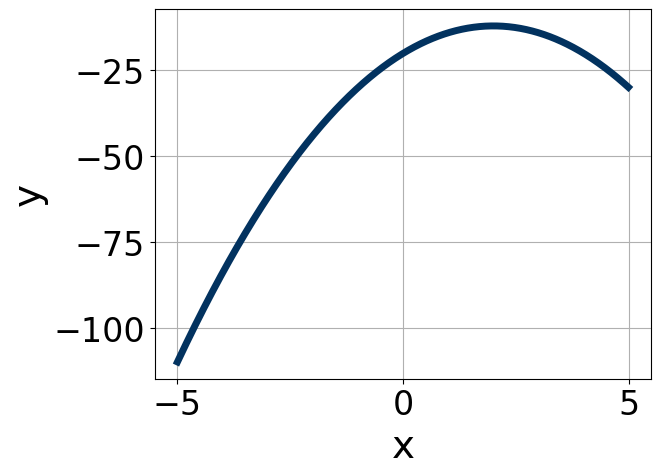
\includegraphics[width = 0.3\textwidth]{../Figures/quadraticEquationToGraphCopyAA.png}\item 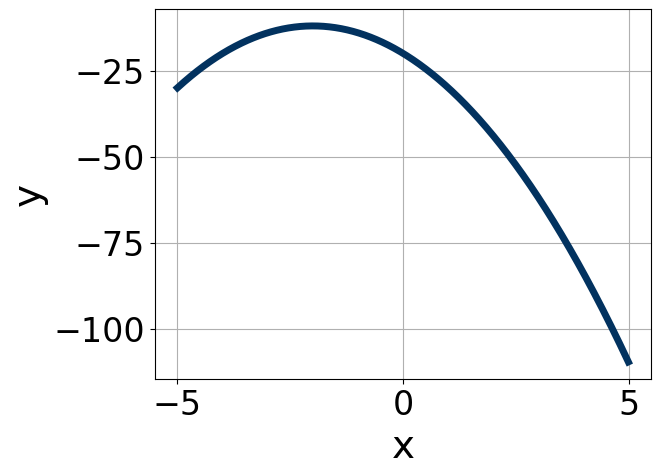
\includegraphics[width = 0.3\textwidth]{../Figures/quadraticEquationToGraphCopyBA.png}\item 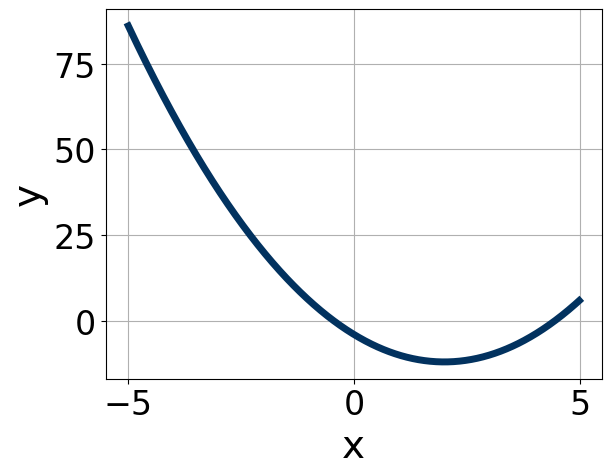
\includegraphics[width = 0.3\textwidth]{../Figures/quadraticEquationToGraphCopyCA.png}\item 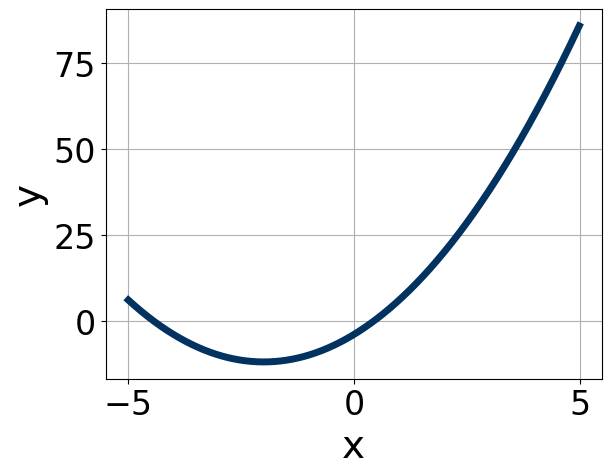
\includegraphics[width = 0.3\textwidth]{../Figures/quadraticEquationToGraphCopyDA.png}\end{multicols}\item None of the above.
\end{enumerate} }
\litem{
Factor the quadratic below. Then, choose the intervals that contain the constants in the form $(ax+b)(cx+d); b \leq d.$\[ 36x^{2} -60 x + 25 \]\begin{enumerate}[label=\Alph*.]
\item \( a \in [17.82, 18.15], \hspace*{5mm} b \in [-11, -2], \hspace*{5mm} c \in [1.94, 3.43], \text{ and } \hspace*{5mm} d \in [-5, -3] \)
\item \( a \in [-0.25, 1.19], \hspace*{5mm} b \in [-31, -21], \hspace*{5mm} c \in [0.36, 1.88], \text{ and } \hspace*{5mm} d \in [-32, -29] \)
\item \( a \in [1.53, 3.89], \hspace*{5mm} b \in [-11, -2], \hspace*{5mm} c \in [17.71, 18.48], \text{ and } \hspace*{5mm} d \in [-5, -3] \)
\item \( a \in [5.77, 6.01], \hspace*{5mm} b \in [-11, -2], \hspace*{5mm} c \in [5.38, 6.44], \text{ and } \hspace*{5mm} d \in [-5, -3] \)
\item \( \text{None of the above.} \)

\end{enumerate} }
\litem{
Factor the quadratic below. Then, choose the intervals that contain the constants in the form $(ax+b)(cx+d); b \leq d.$\[ 54x^{2} -75 x + 25 \]\begin{enumerate}[label=\Alph*.]
\item \( a \in [17.5, 20.9], \hspace*{5mm} b \in [-5, -2], \hspace*{5mm} c \in [1.7, 3.1], \text{ and } \hspace*{5mm} d \in [-5, -4] \)
\item \( a \in [8, 9.6], \hspace*{5mm} b \in [-5, -2], \hspace*{5mm} c \in [5.7, 7.9], \text{ and } \hspace*{5mm} d \in [-5, -4] \)
\item \( a \in [2.4, 4.5], \hspace*{5mm} b \in [-5, -2], \hspace*{5mm} c \in [17.2, 21.4], \text{ and } \hspace*{5mm} d \in [-5, -4] \)
\item \( a \in [0.3, 2], \hspace*{5mm} b \in [-45, -39], \hspace*{5mm} c \in [-0.1, 2.7], \text{ and } \hspace*{5mm} d \in [-32, -29] \)
\item \( \text{None of the above.} \)

\end{enumerate} }
\litem{
Graph the equation below.\[ f(x) = -(x-2)^2 - 15 \]\begin{enumerate}[label=\Alph*.]
\begin{multicols}{2}\item 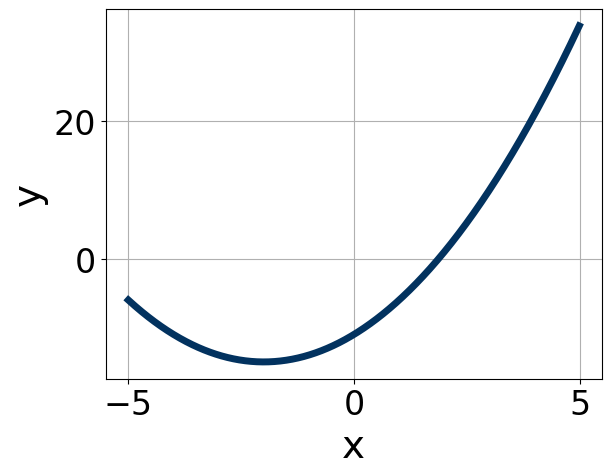
\includegraphics[width = 0.3\textwidth]{../Figures/quadraticEquationToGraphAA.png}\item 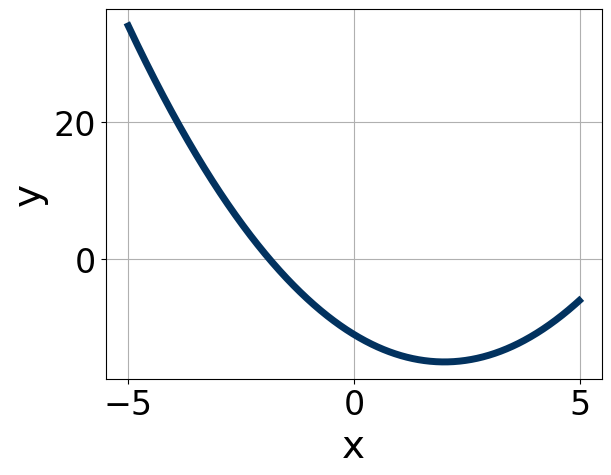
\includegraphics[width = 0.3\textwidth]{../Figures/quadraticEquationToGraphBA.png}\item 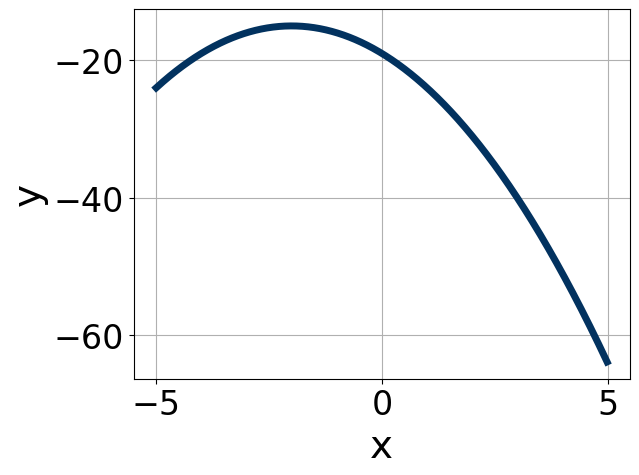
\includegraphics[width = 0.3\textwidth]{../Figures/quadraticEquationToGraphCA.png}\item 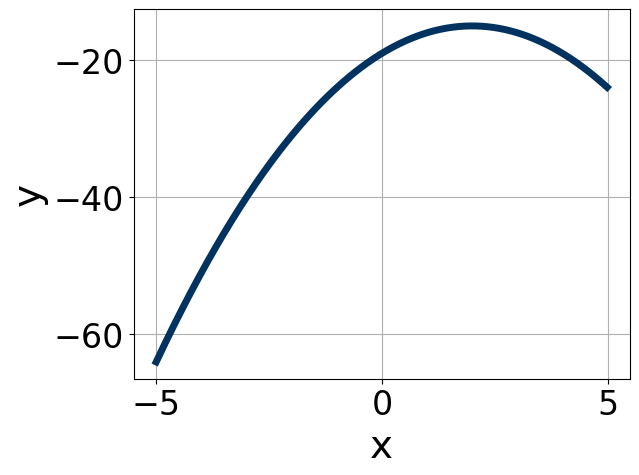
\includegraphics[width = 0.3\textwidth]{../Figures/quadraticEquationToGraphDA.png}\end{multicols}\item None of the above.
\end{enumerate} }
\litem{
Solve the quadratic equation below. Then, choose the intervals that the solutions belong to, with $x_1 \leq x_2$ (if they exist).\[ -12x^{2} -10 x + 5 = 0 \]\begin{enumerate}[label=\Alph*.]
\item \( x_1 \in [-0.5, 0.7] \text{ and } x_2 \in [0.5, 2] \)
\item \( x_1 \in [-6.2, -2.8] \text{ and } x_2 \in [12.2, 14.3] \)
\item \( x_1 \in [-1.5, -0.4] \text{ and } x_2 \in [-0.3, 1] \)
\item \( x_1 \in [-20.1, -18] \text{ and } x_2 \in [16.5, 18.7] \)
\item \( \text{There are no Real solutions.} \)

\end{enumerate} }
\litem{
Solve the quadratic equation below. Then, choose the intervals that the solutions belong to, with $x_1 \leq x_2$ (if they exist).\[ 20x^{2} -12 x -4 = 0 \]\begin{enumerate}[label=\Alph*.]
\item \( x_1 \in [-21.27, -20.75] \text{ and } x_2 \in [21.6, 22.6] \)
\item \( x_1 \in [-4.87, -4.48] \text{ and } x_2 \in [15, 18.5] \)
\item \( x_1 \in [-1.53, -0.44] \text{ and } x_2 \in [0.1, 0.4] \)
\item \( x_1 \in [-0.54, 0.22] \text{ and } x_2 \in [0.6, 2.1] \)
\item \( \text{There are no Real solutions.} \)

\end{enumerate} }
\litem{
Solve the quadratic equation below. Then, choose the intervals that the solutions $x_1$ and $x_2$ belong to, with $x_1 \leq x_2$.\[ 20x^{2} -69 x + 54 = 0 \]\begin{enumerate}[label=\Alph*.]
\item \( x_1 \in [0.71, 0.75] \text{ and } x_2 \in [3.14, 4.04] \)
\item \( x_1 \in [0.58, 0.61] \text{ and } x_2 \in [3.76, 4.87] \)
\item \( x_1 \in [23.99, 24.03] \text{ and } x_2 \in [44.08, 45.72] \)
\item \( x_1 \in [1.16, 1.22] \text{ and } x_2 \in [1.85, 2.93] \)
\item \( x_1 \in [0.45, 0.46] \text{ and } x_2 \in [5.51, 6.52] \)

\end{enumerate} }
\litem{
Solve the quadratic equation below. Then, choose the intervals that the solutions $x_1$ and $x_2$ belong to, with $x_1 \leq x_2$.\[ 15x^{2} +38 x + 24 = 0 \]\begin{enumerate}[label=\Alph*.]
\item \( x_1 \in [-2.78, -2.65] \text{ and } x_2 \in [-0.62, -0.51] \)
\item \( x_1 \in [-2.6, -1.67] \text{ and } x_2 \in [-0.74, -0.61] \)
\item \( x_1 \in [-6.56, -5.86] \text{ and } x_2 \in [-0.27, -0.26] \)
\item \( x_1 \in [-20.18, -19.34] \text{ and } x_2 \in [-18.08, -17.99] \)
\item \( x_1 \in [-1.67, -0.95] \text{ and } x_2 \in [-1.29, -1.18] \)

\end{enumerate} }
\litem{
Write the equation of the graph presented below in the form $f(x)=ax^2+bx+c$, assuming  $a=1$ or $a=-1$. Then, choose the intervals that $a, b,$ and $c$ belong to.
\begin{center}
    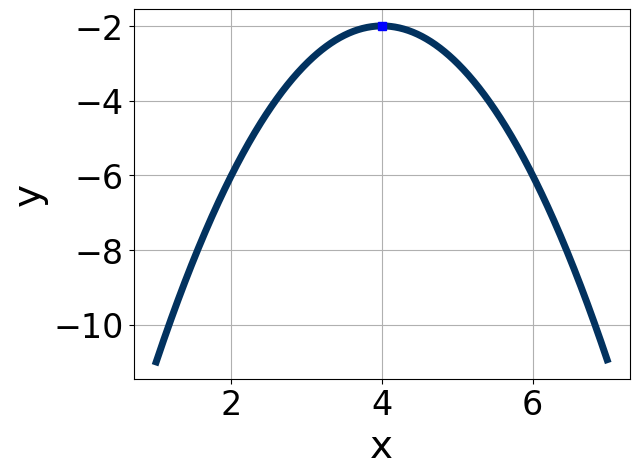
\includegraphics[width=0.5\textwidth]{../Figures/quadraticGraphToEquationA.png}
\end{center}
\begin{enumerate}[label=\Alph*.]
\item \( a \in [-1.6, -0.8], \hspace*{5mm} b \in [7, 13], \text{ and } \hspace*{5mm} c \in [-19, -17] \)
\item \( a \in [-1.6, -0.8], \hspace*{5mm} b \in [-8, -5], \text{ and } \hspace*{5mm} c \in [-15, -11] \)
\item \( a \in [-1.6, -0.8], \hspace*{5mm} b \in [-8, -5], \text{ and } \hspace*{5mm} c \in [-19, -17] \)
\item \( a \in [-0.2, 1.6], \hspace*{5mm} b \in [7, 13], \text{ and } \hspace*{5mm} c \in [13, 18] \)
\item \( a \in [-0.2, 1.6], \hspace*{5mm} b \in [-8, -5], \text{ and } \hspace*{5mm} c \in [13, 18] \)

\end{enumerate} }
\litem{
Write the equation of the graph presented below in the form $f(x)=ax^2+bx+c$, assuming  $a=1$ or $a=-1$. Then, choose the intervals that $a, b,$ and $c$ belong to.
\begin{center}
    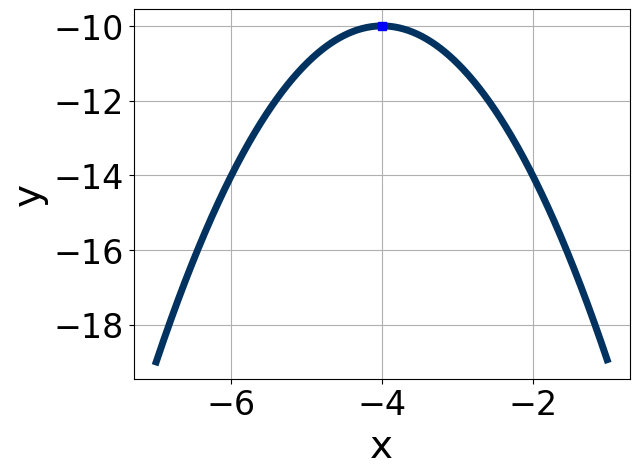
\includegraphics[width=0.5\textwidth]{../Figures/quadraticGraphToEquationCopyA.png}
\end{center}
\begin{enumerate}[label=\Alph*.]
\item \( a \in [1, 3], \hspace*{5mm} b \in [-10, -7], \text{ and } \hspace*{5mm} c \in [5, 9] \)
\item \( a \in [1, 3], \hspace*{5mm} b \in [6, 12], \text{ and } \hspace*{5mm} c \in [5, 9] \)
\item \( a \in [-3, 0], \hspace*{5mm} b \in [6, 12], \text{ and } \hspace*{5mm} c \in [-7, -1] \)
\item \( a \in [-3, 0], \hspace*{5mm} b \in [6, 12], \text{ and } \hspace*{5mm} c \in [-26, -23] \)
\item \( a \in [-3, 0], \hspace*{5mm} b \in [-10, -7], \text{ and } \hspace*{5mm} c \in [-26, -23] \)

\end{enumerate} }
\end{enumerate}

\end{document}